\documentclass[a4paper,
12pt,
BCOR12mm,
]{scrartcl}
%scrreport
\usepackage[ngerman]{babel}
\usepackage[utf8]{inputenc}
\usepackage[T1]{fontenc}
\usepackage{url}
\usepackage[pdftex]{graphicx}
\usepackage{listingsutf8}
\usepackage{grffile}
\usepackage{epstopdf}
\usepackage{subfigure}
\usepackage[a4paper,left=23mm,right=23mm, top=33mm, bottom=66mm]{geometry}
% lstlisting settings
\lstset{
showspaces=false,
breaklines=true,
breakindent=0pt,
frame=single,
language=C,
extendedchars=true,
inputencoding=utf8/latin1,
identifierstyle=\ttfamily,
basicstyle=\tiny,
numbers=left,
numberstyle=\tiny,
}

\title{APUVS, Blatt 4}
\author{Jan Fajerski and Kai Warncke and Magnus Müller}

\begin{document}
% NOTE: compile with pdflatex --shell-escape main.tex

\maketitle 

\section*{Aufgabe 4.1}
\subsection{Testmaschine}
\begin{verbatim}
% uname -a
Linux centraldogma 2.6.35-ARCH #1 SMP PREEMPT Sat Oct 30 21:22:26 CEST 2010
	x86_64 Intel(R) Core(TM) i5 CPU M 520 @ 2.40GHz GenuineIntel GNU/Linux

% cat /proc/meminfo
MemTotal:        3848056 kB
MemFree:         1889880 kB
Buffers:          352748 kB
Cached:           541128 kB
[...]
\end{verbatim}

\subsubsection*{1.}
Auf unserem Testsystem werden standardmäßig 4 Threads verwendet. Dies entspricht auch der
in \url{http://ark.intel.com/Product.aspx?id=47341} angegebenen Anzahl von gleichzeitig
möglichen Threads (wobei hierbei Hyperthreading genutzt wird und nicht echte
Parallelität auf 4 Kernen).

\subsubsection*{2.}
Unser Aufrufskript \verb|call.sh| auf Seite \pageref{src:call} ruft zwei Programme auf:
\begin{itemize}
	\item \verb|summation|, vgl. Seite \pageref{src:sum}
	\item \verb|summation_ascending_nums|, vgl. Seite \pageref{src:ascend}
\end{itemize}

\verb|summation| führt die in der Aufgabenstellung beschriebene Berechnung durch
(Summation $\sum_{i=1}^{n} 1 = n$). \verb|summation_ascending_nums| berechnet hingegen
$\sum_{i=1}^{n} i = \frac{n (n+1)}{2}$. \\

Überraschenderweise kommt es bei beiden Programmen zu großen Unterschieden in den
Laufzeiten, je nach Anzahl von Threads und Arraygröße. Die Diagramme \ref{fig:summation_1_3},
\ref{fig:summation_4_6} und \ref{fig:summation_7_10} stellen für \verb|summation| den
Median der Durchlaufzeiten von 30 Durchläufen dar, wobei jeder Durchlauf eine Summation eines
Arrays mit gegebener Anzahl an Elementen und mit einer festen Anzahl von Threads (gesetzt
über \verb|omp_set_num_threads()|) durchführt. Für \verb|summation_ascending_nums| sind dies
entsprechend die Abbildungen \ref{fig:ascending_1_3}, \ref{fig:ascending_4_6} und
\ref{fig:ascending_7_10}. Wir haben hier mit Absicht die Darstellung des Medians gewählt,
da eine Durchschnittsbildung aufgrund der sehr großen Varianz der Ausführungszeiten zu
stark durch Ausreißer dominiert wird. \\
Betrachtet man hierzu die Abbildungen \ref{fig:summation_4threads_avg},
\ref{fig:summation_4threads_slowest} und \ref{fig:summation_4threads_median}, so ergibt
sich, dass die Ausführung von \verb|summation| bei Verwendung von 4 Threads
\emph{oft} schneller ist als bei einer anderen Anzahl von Threads. Jedoch kommt es immer wieder zu sehr starken
Ausreißern, wie in Abbildung \ref{fig:summation_4threads_slowest} dargestellt wird. Durch
Ausreißer im zweistelligen Millisekundenbereich (und somit einem Unterschied in mehreren
Größenordnungen) wird der Durchschnittswert zu sehr verfälscht, als dass dieser noch eine
starke Aussagekraft hätte.\\
Trotz der mehrfachen Ausführung jedes einzelnen Aufrufs (jeder Aufruf wird 30 mal
wiederholt, siehe Aufrufskript Seite \pageref{src:call}) können temporäre Seiteneffekte
nicht ausgeschlossen werden. \\
Anhand des Medians lässt sich aber mit einiger Sicherheit festhalten, dass die
Verwendung von vier Threads auf der gegebenen Testmaschine zumeist das schnellste Ergebnis
liefert. Bei wachsender Arraygröße benötigt das Programm in der Ausführung auch mehr Zeit.
Wie in den Abbildungen zu sehen ist, ist das Anstieg aber nahezu linear. Wie in Abbildung
\ref{fig:summation_4_6} benötigt die Ausführung von \verb|summation| mit 4 Threads am
wenigsten Zeit, wobei bei kleineren Arraygrößen (vgl. hierzu die Diagramme zu den
Ausführungszeiten von \verb|summation_ascending_nums|) die Verwendung eines einzelnen
Threads durchaus noch schneller sein kann. Somit bestimmt nicht nur die Anzahl der Threads
die Ausführungszeit, sondern auch die Problemgröße.


% some graphs
\begin{figure}[!h]
	\begin{center}
		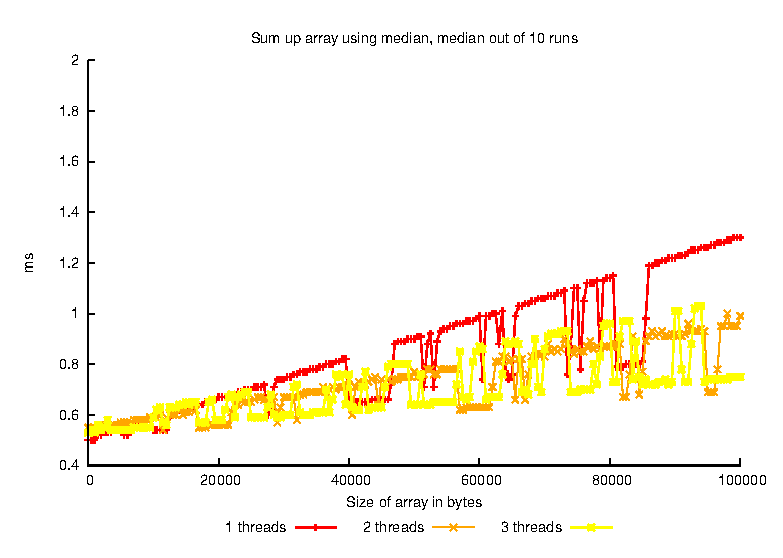
\includegraphics[width=0.5\textwidth]{../a_4_1/graphs/summation_median_1st}
	\end{center}
	\caption{Summation mit 1-3 Threads}
	\label{fig:summation_1_3}
\end{figure}
\begin{figure}[!h]
	\begin{center}
		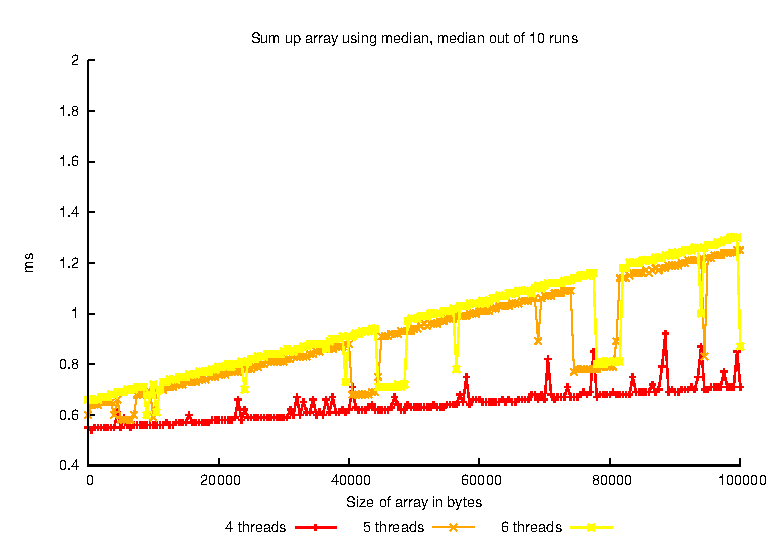
\includegraphics[width=0.5\textwidth]{../a_4_1/graphs/summation_median_2nd}
	\end{center}
	\caption{Summation mit 4-6 Threads}
	\label{fig:summation_4_6}
\end{figure}
\begin{figure}[!h]
	\begin{center}
		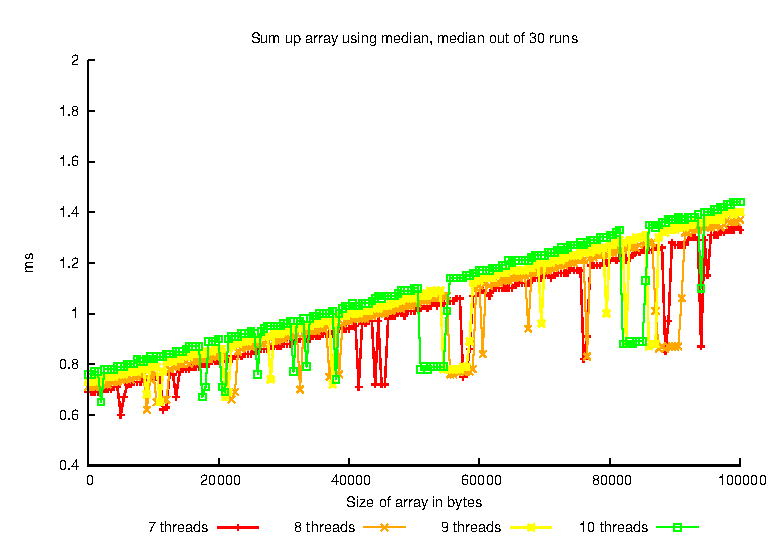
\includegraphics[width=0.5\textwidth]{../a_4_1/graphs/summation_median_3rd}
	\end{center}
	\caption{Summation mit 7-10 Threads}
	\label{fig:summation_7_10}
\end{figure}

\begin{figure}[!h]
	\begin{center}
		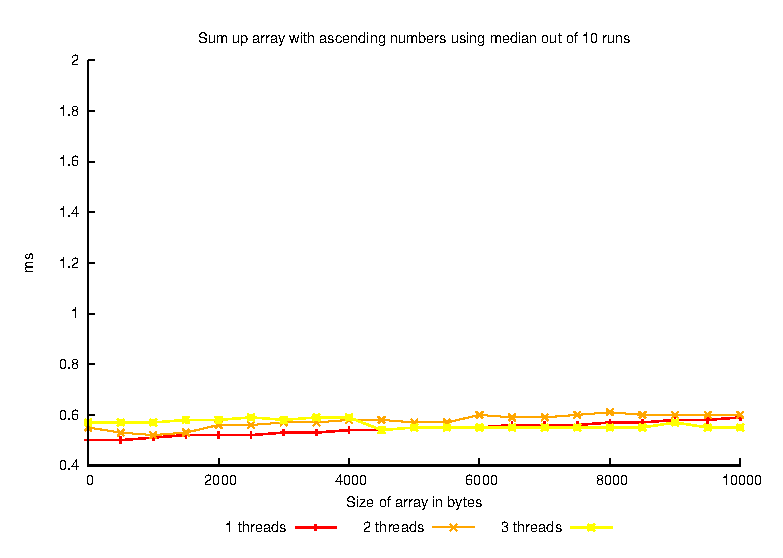
\includegraphics[width=0.5\textwidth]{../a_4_1/graphs/ascending_median_1st}
	\end{center}
	\caption{Summation aufsteigender Zahlen mit 1-3 Threads}
	\label{fig:ascending_1_3}
\end{figure}
\begin{figure}[!h]
	\begin{center}
		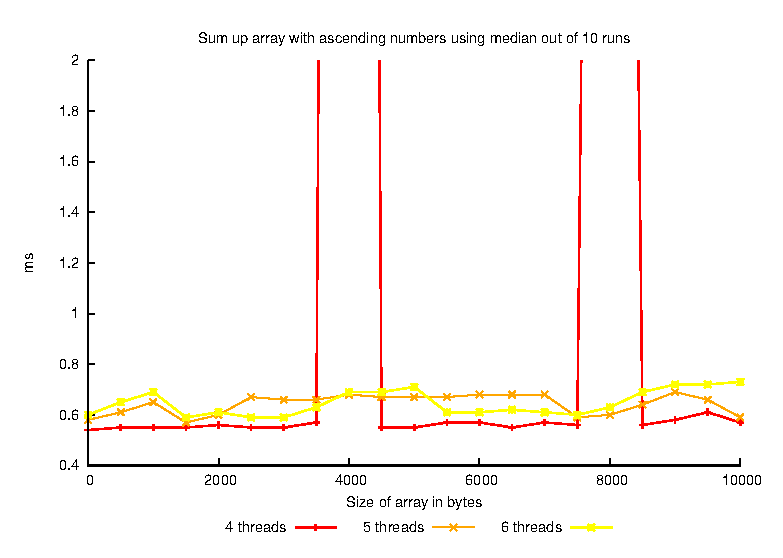
\includegraphics[width=0.5\textwidth]{../a_4_1/graphs/ascending_median_2nd}
	\end{center}
	\caption{Summation aufsteigender Zahlen mit 4-6 Threads}
	\label{fig:ascending_4_6}
\end{figure}
\begin{figure}[!h]
	\begin{center}
		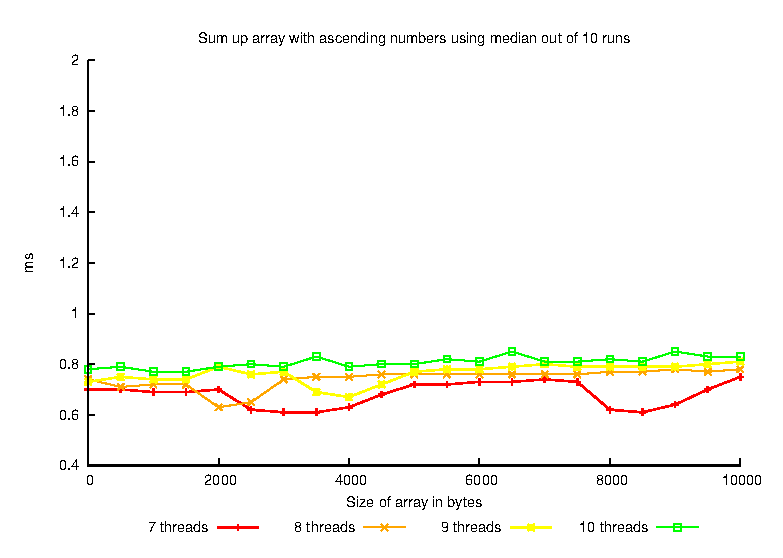
\includegraphics[width=0.5\textwidth]{../a_4_1/graphs/ascending_median_3rd}
	\end{center}
	\caption{Summation aufsteigender Zahlen mit 7-10 Threads}
	\label{fig:ascending_7_10}
\end{figure}

\begin{figure}[!h]
	\begin{center}
		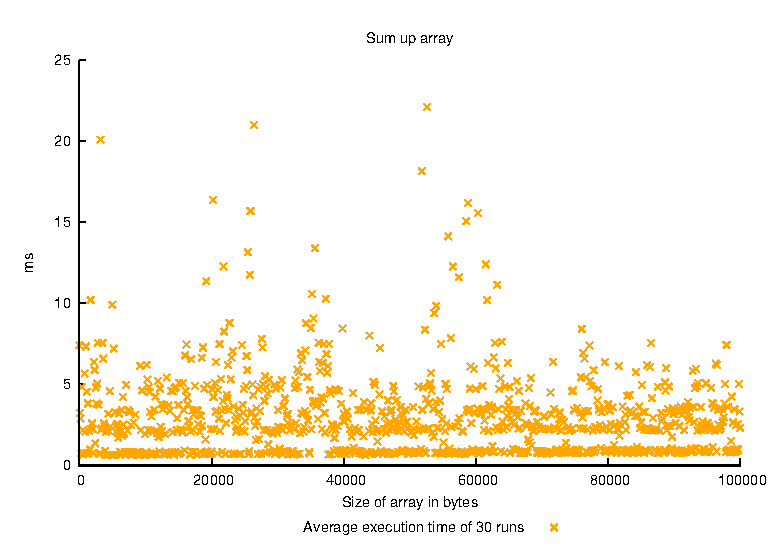
\includegraphics[width=0.5\textwidth]{../a_4_1/graphs/4_summation_average.eps}
	\end{center}
	\caption{Summation mit 4 Threads, hohe Auflösung}
	\label{fig:summation_4threads_avg}
\end{figure}
\begin{figure}[!h]
	\begin{center}
		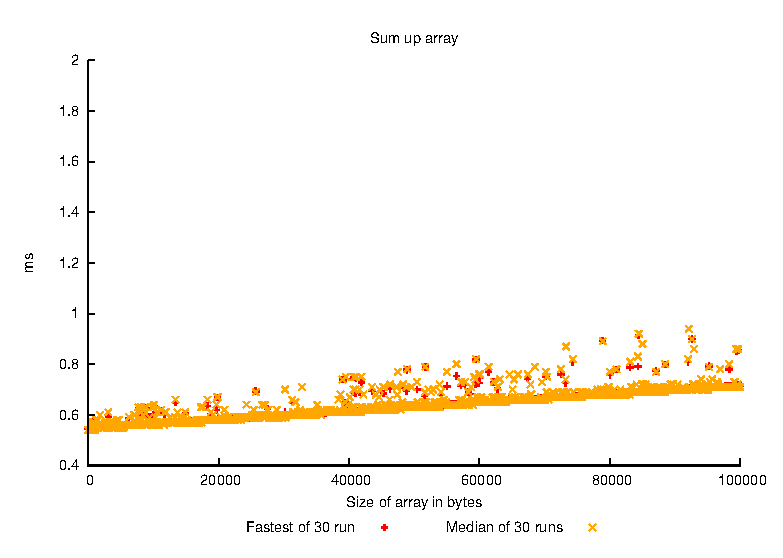
\includegraphics[width=0.5\textwidth]{../a_4_1/graphs/4_summation_fastestandmedian.eps}
	\end{center}
	\caption{Summation mit 4 Threads, hohe Auflösung, schnellster Run und Median}
	\label{fig:summation_4threads_median}
\end{figure}
\begin{figure}[!h]
	\begin{center}
		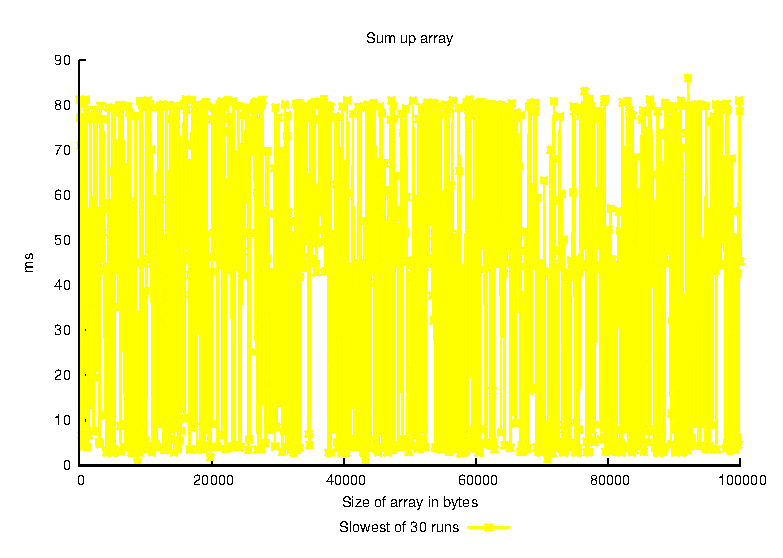
\includegraphics[width=0.5\textwidth]{../a_4_1/graphs/4_summation_slowest.eps}
	\end{center}
	\caption{Summation mit 4 Threads, hohe Auflösung, langsamster Run}
	\label{fig:summation_4threads_slowest}
\end{figure}
\clearpage

\section*{Aufgabe 4.2}
Die Dining Philosophers wurden mit Java und \verb|synchronized| Methoden
implementiert (siehe Quelltexte \ref{src:java}. Das Programm produziert ein
Deadlock. Zur Auflösung des Deadlocks ist bereits ein Codefragment im Quelltext
\ref{src:java} vorbereitet und kommentiert. 
Der Deadlock wird hervor gerufen, da alle Philosophen als erstes versuchen die
linke Gabel aufzunehmen. Haben sie dies geschafft, versuchen sie dir rechte
Gabel aufzunehmen. Da die Methode \verb|Fork.take()| die private
synchronized-Methode \verb|Fork.changeStatus()| aufruft sobald die Gabel
verfügbar ist (und so lange eine busy-wait macht), sind alle 4
Coffman-Bedingungen erfüllt:\\
\begin{tabular}{lp{11cm}}
  No Preemption     & Die Philosophen müssen selbst die Gabeln wieder freigeben \\
  Hold and Wait     & Hat ein Philosoph die linke Gabel aufgenommen, behält er sie solange, bis er auch die rechte Gabel hat um zu essen. \\
  Mutual Exclusion  & Jede Gabel kann nur im Besitz eines Philosophen sein. \\
  Circular Wait     & Die zirkuläre Abhängigkeit ist natürlich im Problem der speisenden Philosophen gegeben und durch die runde Tafel illustiert.
\end{tabular} \\
Der Deadlock ist sehr leicht zu vermeiden. Wie im Quelltext beschrieben ist es
ausreichend, vor dem Aufnehmen der rechten Gabel zu testen, ob diese in
Benutzung ist. Ist sie weg, wird auch die linke Gabel wieder auf den Tisch
gelegt. Damit ist die Hold-and-Wait Bedingung gebrochen und es kann nicht mehr
zu einem Deadlock kommen. Es kann allerdings dazu kommen, dass ein Philosoph
verhungert.
Der Ablauf mit Deadlock \footnote{die Aufrufe von sleep() erzeugen den Deadlock
gleich am Anfang, sonst dauert es unter Umständen sehr lange}:
\begin{verbatim}
Machiaveli got his left fork...WOOHOO
Russel got his left fork...WOOHOO
Leibnitz got his left fork...WOOHOO
Kant got his left fork...WOOHOO
Sokrates got his left fork...WOOHOO
\end{verbatim}
Ohne Deadlock ist ein mögliches Ablaufprotokoll:
\begin{verbatim}
Machiaveli got his left fork...WOOHOO
Russel got his left fork...WOOHOO
Leibnitz got his left fork...WOOHOO
Kant got his left fork...WOOHOO
Sokrates got his left fork...WOOHOO
Machiaveli puts his left fork down....right fork is used
Leibnitz puts his left fork down....right fork is used
Russel got his right fork...WOOHOO
Russel is eating...nomnomnomnomnomnomnomnomnomnomn
Sokrates puts his left fork down....right fork is used
Kant puts his left fork down....right fork is used
Leibnitz got his left fork...WOOHOO
Sokrates got his left fork...WOOHOO
Kant got his left fork...WOOHOO
Leibnitz puts his left fork down....right fork is used
Sokrates puts his left fork down....right fork is used
Kant got his right fork...WOOHOO
Kant is eating...nomnomnomnomnomnomnomnomnomnomn
Russel puts down his dirty forks
Russel got his left fork...WOOHOO
Leibnitz got his left fork...WOOHOO
\end{verbatim}
\section*{Aufgabe 4.3}
Vorteile von \emph{DRAGON} gegenüber \emph{MESI}:
\begin{itemize}
	\item Kürzere Zugriffszeit: Da bei einer Schreiboperation Werte immer in allen Caches
		geändert werden, können Daten in den Caches nicht ungültig werden. Dadurch kommt es 
		nicht zu späteren cachemisses.\footnote{Falls ein Datum nicht geteilt wird, also nur
		ein Prozessor dieses im Cache haben will, dann muss kein Update durchgeführt werden.
		Vergleiche hierzu Folie 27.}
	\item \emph{DRAGON} spart Bandbreite gegenüber \emph{MESI}: Da bei einem Update nur das
		eigentliche Datum auf den Bus gegeben werden muss,\footnote{Vgl. vorherige Fußnote} und nicht der gesamte Block wie bei
		\emph{MESI}, wird weniger Bandbreite "`verschwendet"'.
\end{itemize}

Neben den genannten Vorteilen hat \emph{DRAGON} aber auch Nachteile:
\begin{itemize}
	\item Unmittelbar aufeinanderfolgende Schreiboperationen eines Prozessors erzeugen unter
		Umständen mehrere Update-Transaktionen (da die Daten über verschiedene Caches "`synchronisiert"`
		werden müssen). Dies steht im Gegensatz zu \emph{MESI}, da ein Prozessor bei
		\emph{MESI} exklusives Schreibrecht hat und dieses behält, bis ein anderer Prozessor
		das exklusive Schreibrecht erhält.
\end{itemize}
\section{Quelltexte}
\subsection{Aufgabe 4.1}
\subsubsection{Aufrufskript}
\label{src:call}
\lstinputlisting[language=Bash]{../a_4_1/call.sh}
 
\subsubsection{Einfache Summation}
\label{src:sum}
\lstinputlisting{../a_4_1/summation.c}
\subsubsection{Summation mit Array aufsteigender Zahlen}
\label{src:ascend}
\lstinputlisting{../a_4_1/summation_ascending_nums.c}

\subsubsection{Berechnung der Zeitdifferenz}
\label{src:messure}
\lstinputlisting{../a_4_1/messuretime.h}
\lstinputlisting{../a_4_1/messuretime.c}

\subsubsection{Ausgabefunktion}
\label{src:basic}
\lstinputlisting{../a_4_1/basic_functions.h}
\lstinputlisting{../a_4_1/basic_functions.c}
\subsection{Aufgabe 4.2}
\subsubsection{Java Quelltexte}
\label{src:java}
\lstinputlisting[language=Java]{../a_4_2/diningphilosophers/Main.java}
\lstinputlisting[language=Java]{../a_4_2/diningphilosophers/Fork.java}
\lstinputlisting[language=Java]{../a_4_2/diningphilosophers/Philosopher.java}

\end{document}
